
%(BEGIN_QUESTION)
% Copyright 2012, Tony R. Kuphaldt, released under the Creative Commons Attribution License (v 1.0)
% This means you may do almost anything with this work of mine, so long as you give me proper credit

Forklar hvordan hvert av følgende trykkinstrumenter virker, og identifiser om hvert instrument bruker prinsippet \textit{bevegelsesbalanse} (motion-balance) eller \textit{kraftbalanse} (force-balance).  Merk at en serie skrå streker ut fra en vertikal eller horisontal linje betyr forankringspunkt, altså at denne flaten står stille:

\vskip 10pt

\noindent
{\bf Eksempel 1:}

$$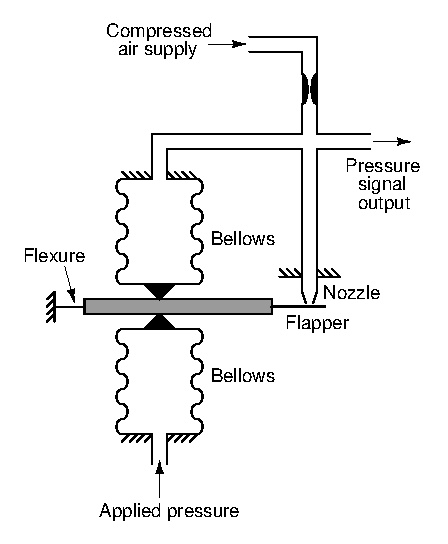
\includegraphics[width=15.5cm]{i00208x01.eps}$$

\vskip 10pt

\filbreak

\noindent
{\bf Eksempel 2:}

$$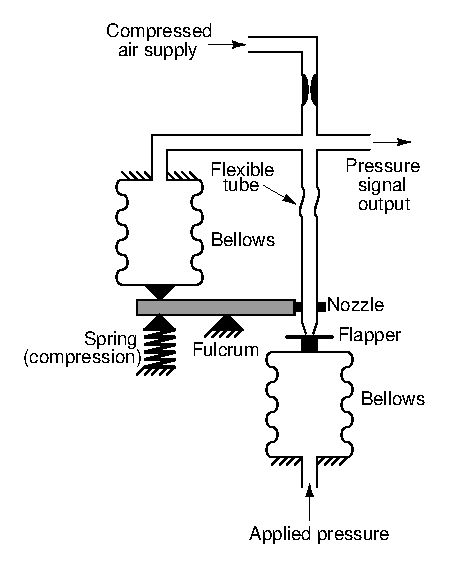
\includegraphics[width=15.5cm]{i00208x02.eps}$$

\vskip 10pt

\filbreak

\noindent
{\bf Eksempel 3:}

$$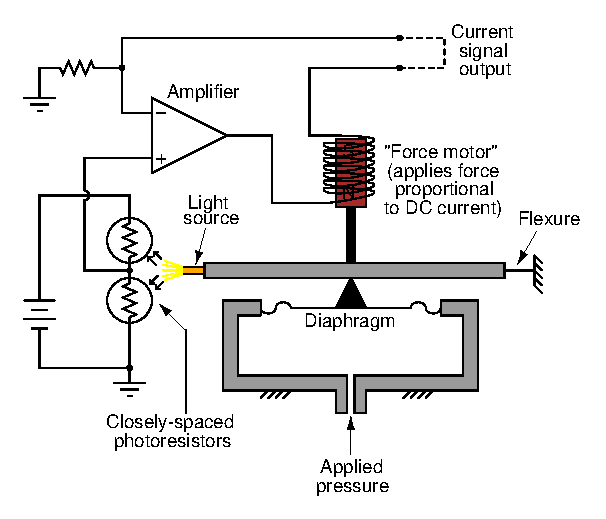
\includegraphics[width=15.5cm]{i00208x03.eps}$$

\vskip 10pt

\filbreak

\noindent
{\bf Eksempel 4:}

$$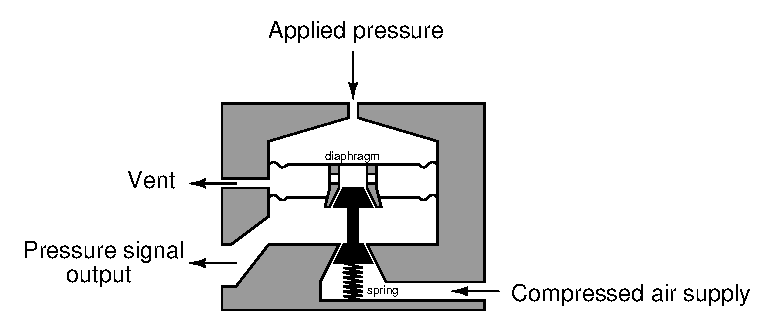
\includegraphics[width=15.5cm]{i00208x04.eps}$$

\vskip 10pt

\filbreak

\noindent
{\bf Eksempel 5:}

$$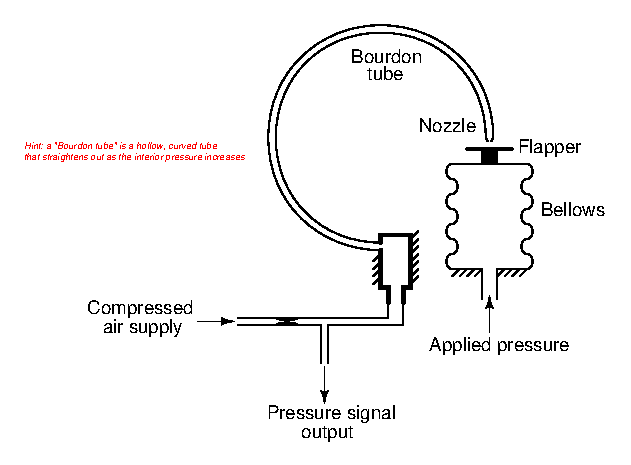
\includegraphics[width=15.5cm]{i00208x05.eps}$$

\vskip 10pt

\filbreak

\noindent
{\bf Eksempel 6:}

$$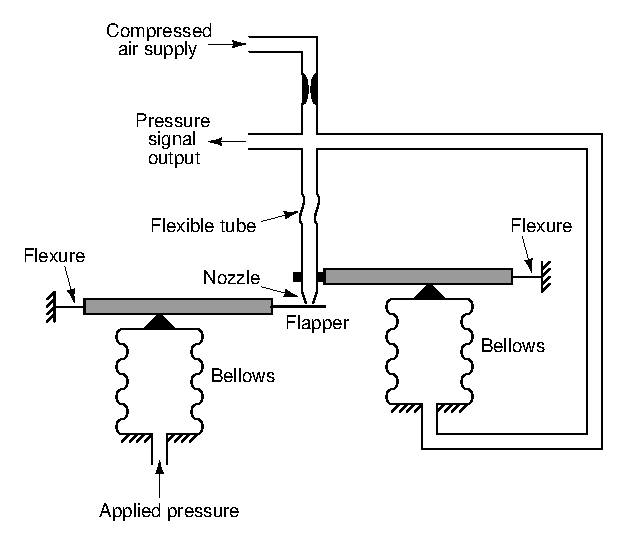
\includegraphics[width=15.5cm]{i00208x06.eps}$$

\vskip 10pt

\filbreak

\noindent
{\bf Eksempel 7:}

$$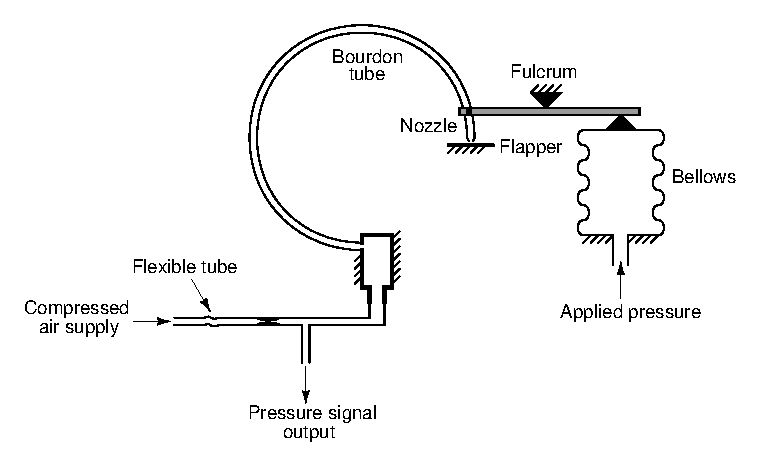
\includegraphics[width=15.5cm]{i00208x07.eps}$$

\vskip 10pt

\filbreak

\noindent
{\bf Eksempel 8:}

$$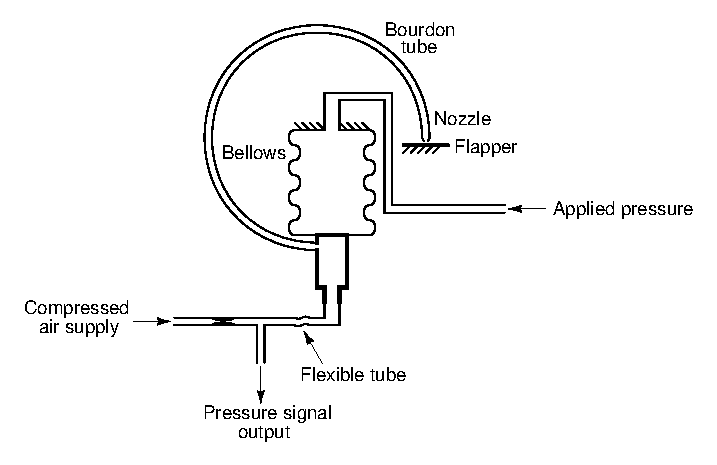
\includegraphics[width=15.5cm]{i00208x08.eps}$$

\vskip 10pt

\filbreak

\noindent
{\bf Eksempel 9:}

$$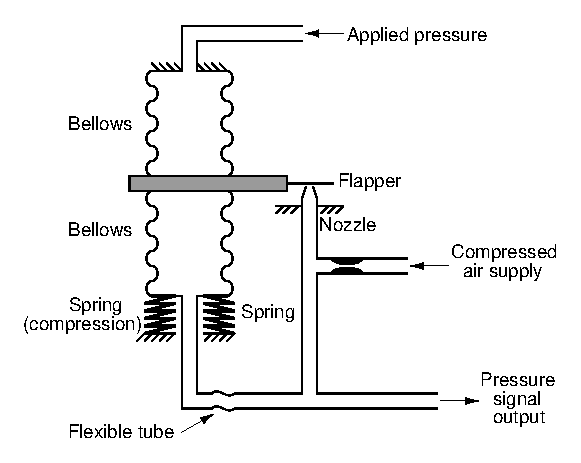
\includegraphics[width=15.5cm]{i00208x09.eps}$$




\vskip 20pt \vbox{\hrule \hbox{\strut \vrule{} {\bf Suggestions for Socratic discussion} \vrule} \hrule}

\begin{itemize}
\item{} Skillet mellom kraftbalanse og bevegelsesbalanse forvirrer ofte studenter.  En vanlig feil er å prøve å memorere kjennetegn for å gjenkjenne mekanismetypen.  En bedre strategi er å \textit{resonnere} gjennom mekanismens drift med ``tankeeksperimenter'' og derfra avgjøre balanseprinsipp.  Hvorfor er memorering dårligere enn tankeeksperiment?
\item{} Hvilken praktisk betydning har det for oss (som teknikere) å vite om en mekanisme er kraft- eller bevegelsesbalansert?
\item{} Identifiser endringer som kan gjøres i hver mekanisme for å endre \textit{nullpunkt}.
\item{} Identifiser endringer som kan gjøres i hver mekanisme for å endre \textit{span}.
\item{} Et nyttig tankeeksperiment er å endre ett aspekt av mekanismen (f.eks. stivere fjær, høyere forsyningstrykk, flytting av orifice) og analysere på nytt hvilke effekter endringen gir.
\end{itemize}

\underbar{file i00208}
%(END_QUESTION)





%(BEGIN_ANSWER)

\begin{itemize}
\item{}(1) Kraftbalanse 
\item{}(2) Bevegelsesbalanse 
\item{}(3) Kraftbalanse 
\item{}(4) Kraftbalanse 
\item{}(5) Bevegelsesbalanse 
\item{}(6) Bevegelsesbalanse 
\item{}(7) Kraftbalanse 
\item{}(8) Bevegelsesbalanse 
\item{}(9) Kraftbalanse 
\end{itemize}

Hovedregelen er at bevegelsesbalanserte instrumenter genererer en \textit{bevegelse} som motvirker en inn-bevegelse for å holde konstant detektorgap (flapper/nozzle), mens kraftbalanserte instrumenter genererer en \textit{kraft} som motvirker en inn-kraft for å holde samme gap konstant.

\vskip 10pt

Eksempel 9 er vanskelig, fordi man kan hevde at det er \textit{bevegelsesbalanse} siden den nedre belgen strekkes når utgangstrykket øker.  Men det avgjørende er at de to belgkreftene motvirker hverandre for å holde flapperen \textit{stasjonær}, og dermed holde konstant flapper/nozzle-gap.  Det er kjennetegnet på kraftbalanse.

Stivheten i fjæren påvirker heller ikke forsterkningen i denne mekanismen, noe den ville gjort i en ekte bevegelsesbalanse (der bevegelsesmengde per trykkøkning er direkte sentral).  Belgkraftene balanserer hverandre ved likevekt uansett hvor mye fjæren må komprimeres underveis.  Hvis mekanismen var ekte bevegelsesbalanse, ville en svakere fjær gitt lavere utgangstrykk fordi mindre trykk trengs for samme vandring.  Her vil svakere fjær gi større bevegelse i nedre belg for samme inngang, men utgangstrykket blir likevel det samme, altså påvirker ikke bevegelseskravet forsterkningen.

%(END_ANSWER)





%(BEGIN_NOTES)

Det fleksible røret i eksempel \#7 er lagt inn bevisst for å lure studenter som knytter bevegelsesbalanse til fleksible rør.  Det fleksible røret i eksempel \#9 er faktisk nødvendig, men endrer ikke at \#9 fortsatt er en kraftbalansemekanisme.

%INDEX% Measurement, pressure: motion- versus force-balance

%(END_NOTES)

